% !TEX root = ../main.tex
\pagebreak[0]
\section{\emph{Square} and \emph{pentagon} configurations}\label{sec:square-and-pentagon-configurations}

\begin{figure}[htbp]
\centering
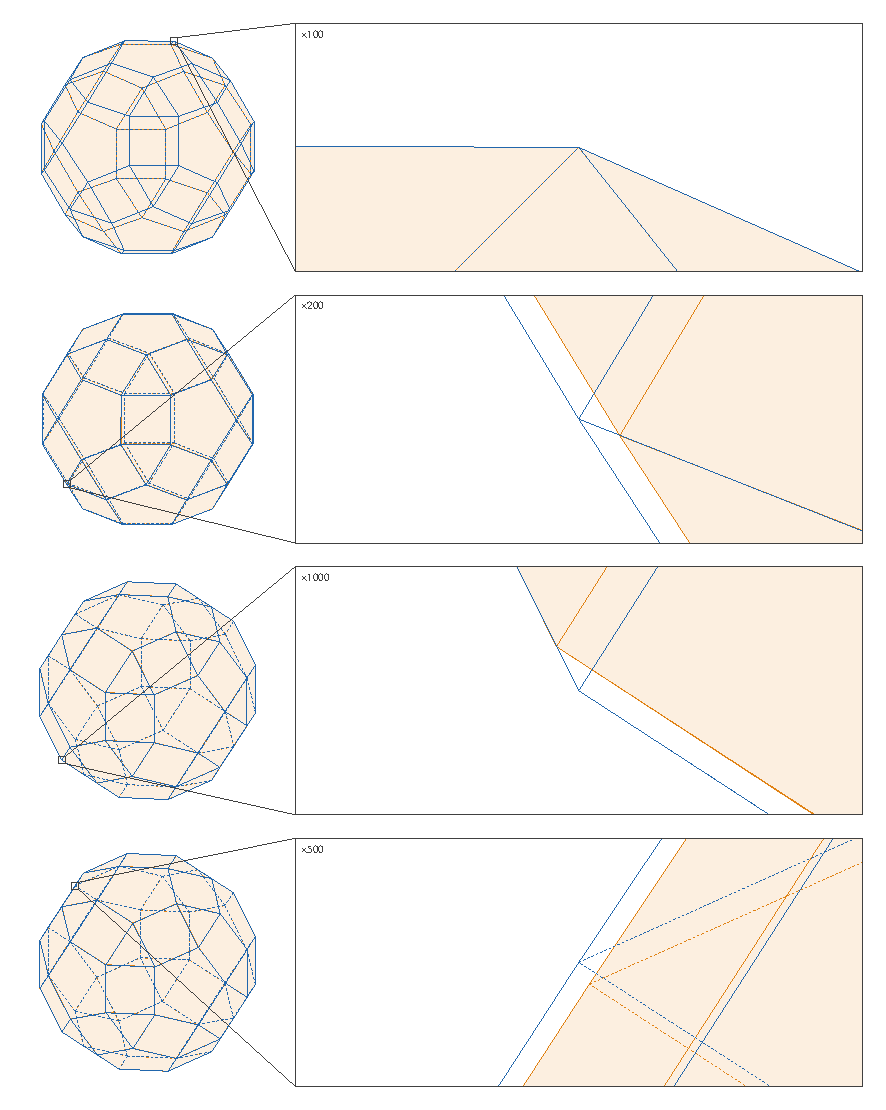
\includegraphics[width=\linewidth]{figures/square-pentagon}
\caption{Near the square configuration (top two rows) and the pentagon configuration (bottom two); the \fc{Hole}{hole (orange)} and the \fc{Plug}{plug (blue)} as in \cref{fig:global-examples}. First: the configuration $[1/16,1/16,(-1/16,1/16,0)]$ of the half-turn family, whose plug shadow and projected edges coincide with the hole's, so that a single wireframe is visible, enlarged $100$ times at a vertex of the outline; it lies outside $D$. Second: the poke configuration $[1/64,1/128,(1/1000,-1/1000,-1/1000)]$, with a plug vertex protruding by about $0.005$ (enlarged $200$ times). Third and fourth: the viewing parameters $(\eta,\xi)=(1/200,-1/400)$ and $(-1/200,-1/400)$ of \cref{subsec:eliminating-the-pentagon-configuration}, on the two sides of the line along which a pentagonal face is seen edge-on, with the rotation $\mathbf r=(1/1000,0,0)$; a different plug vertex protrudes on each side (enlarged $1000$ and $500$ times).}
\label{fig:square-pentagon-examples}
\end{figure}

The two viewing directions left out by the Local component belong to two
aligned configurations. We call the aligned configuration with
$(s,t)=(0,0)$ the \emph{square} configuration: its viewing line passes
through opposite square faces. The second, the \emph{pentagon}
configuration, has
\begin{equation}\label{eq:pentagon-viewing-parameters}
  (s,t)=\left(\frac{-5+3\sqrt5}{10},\frac{5-\sqrt5}{10}\right),
\end{equation}
where the boundary $\varphi s+\varphi^2t=1$ of the viewing triangle meets
the line $s=(-1+\varphi)t$, along which a pentagonal face with normal
$(1,1-\varphi,0)$ is seen edge-on.

Three things make these configurations harder than the other aligned
ones, and the rest of the section deals with them in turn.
\begin{enumerate}
  \item At both, for every vertex and supporting line valid near the special
    viewing direction, the initial outward motion vanishes for some
    directions of rotation, and dividing out the size of
    the rotation is not enough. \emph{Point zooms}, below, divide out a
    second distance: the distance of the viewing parameters from those of
    the special configuration.
  \item At the square configuration, a family of touch configurations with
    nonzero rotation reaches the aligned configuration. The fold
    inequalities of \cref{eq:reduced-domain} remove it
    (\cref{subsec:eliminating-the-square-configuration}).
  \item At the pentagon configuration, the vertices of the edge-on face that
    form the silhouette differ on the two sides of the edge-on line, and so
    do the useful supports (\cref{subsec:eliminating-the-pentagon-configuration}).
\end{enumerate}
Both configurations are handled by one further component, the
\emph{Exotic} component. Like the Local component, it eliminates a
search box by checking that the box lies in the covered set of a zoom
cover that was checked once, before the search. It has two covers here,
one around each configuration, and six more in
\cref{sec:arc-configurations,sec:endpoint-and-crossing-configurations}.

\paragraph{Why one distance is not enough.}
A model shows the difficulty. Let $x\ge0$ measure how far the viewing
parameters are from those of the special configuration, and let $y\ge0$
be the size of the rotation. Suppose a witness behaves like
\[
  p=y(x+y).
\]
A face zoom divides by $y$ and leaves $x+y$, which is positive except at
$x=y=0$, where it vanishes. No zoom cell containing the special
configuration can then pass the test of \cref{lem:zoom-lemma}, however
small. The Local component meets exactly this behaviour at the square and
pentagon configurations: in the directions of rotation described in
\cref{subsec:range-and-exotic-viewing-directions}, the initial
outward motion of every projected vertex, measured against any support
valid near the special configuration, is proportional to $x$.

\paragraph{Point zooms.}
The remedy is to measure the rotation relative to $x$, using two families
of zooms around the special configuration (\cref{fig:toy-zoom}).
\begin{itemize}
  \item In \emph{family A}, the rotation is at most $\rho_0$ times the
    distance of the viewing parameters: that distance is $\mu$, and the
    rotation has size $\rho\mu$ with $0\le\rho\le\rho_0$. Both $\mu$ and
    $\rho$ are distance coordinates. In the model, $p=\mu^2\rho(1+\rho)$.
  \item In \emph{family B}, the rotation is larger: its size is $\delta$ and
    the distance of the viewing parameters is $b\delta$ with
    $0\le b\le1/\rho_0$. The distance coordinate is $\delta$. In the model,
    $p=\delta^2(b+1)$.
\end{itemize}
After division by the zoom factors $\mu^2\rho$ and $\delta^2$, both
quotients are at least one throughout their zoom boxes, including the
special configuration itself, which has become the whole face $\mu=0$ or
$\delta=0$. The ratio $\rho_0>0$ is a parameter; any positive value works in
the model.

\begin{figure}[htbp]
\centering
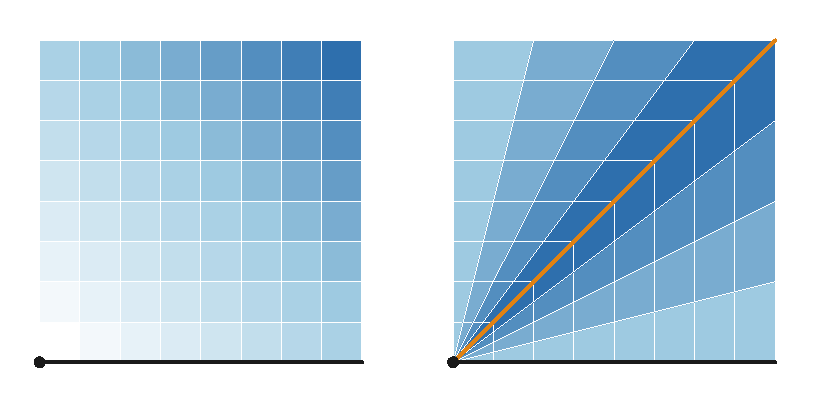
\includegraphics[width=0.9\linewidth]{figures/toy-zoom}
\caption{The model $p=y(x+y)$: the distance $x\ge0$ of the viewing parameters horizontally and the size $y\ge0$ of the rotation vertically, both in $[0,1]$; the no-fit set $y=0$ is the black line and the special configuration the black dot. Each cell is shaded by the smallest value of its quotient, from white for $0$ to \fc{Quotient}{dark blue for $2$}. Left: the cells of a face zoom, which divides by $y$; the quotient $x+y$ fades to $0$ at the special configuration, so the cell there fails however small it is. Right: the point zooms with $\rho_0=1$. Below \fc{Hole}{the diagonal (orange)}, family A, with the segments of constant distance $\mu$ and the rays of constant ratio $\rho$; above it, family B, with the segments of constant rotation size $\delta$ and the rays of constant ratio $b$. The quotients $1+\rho$ and $1+b$ are at least $1$ on every cell, including the cells at the special configuration.}
\label{fig:toy-zoom}
\end{figure}

In general, we use base and offset coordinates as for the tube zooms of
\cref{subsec:the-zoom-lemma}, now around a point: the special configuration
is $\mathbf z_b=\mathbf z_o=\mathbf0$, and the configurations with
$\mathbf z_o=\mathbf0$ lie in the no-fit set. Both parts are normalised on
the faces of boxes: the offsets on the faces of a box
$\Phi\subseteq{[-1,1]}^m$, and the base directions on the faces of a box
$\Sigma\subseteq{[-1,1]}^{5-m}$, each with sides $[-1,0]$, $[0,1]$ or
$[-1,1]$.

Given a base radius $\mu_{\max}$, an offset radius $\delta_{\max}$ and the
ratio $\rho_0$, the \emph{point zooms} are
\begin{itemize}
  \item $\mathcal A_{G,F}$, for each face $G$ of $\Sigma$ and $F$ of $\Phi$:
    $\mathbf z_b=\mu\widehat{\mathbf b}$ and
    $\mathbf z_o=\rho\mu\widehat{\mathbf f}$, with $\widehat{\mathbf b}\in G$,
    $\widehat{\mathbf f}\in F$, $0\le\mu\le\mu_{\max}$ and $0\le\rho\le\rho_0$;
  \item $\mathcal B_F$, for each face $F$ of $\Phi$: $\mathbf z_b=\delta\mathbf b$
    and $\mathbf z_o=\delta\widehat{\mathbf f}$, with $\widehat{\mathbf f}\in F$,
    $0\le\delta\le\delta_{\max}$ and $\mathbf b$ in the cone of $\Sigma$ with
    $\lVert\mathbf b\rVert_\infty\le1/\rho_0$.
\end{itemize}
The free coordinates of $\widehat{\mathbf b}$ and $\widehat{\mathbf f}$ on
their faces are zoom coordinates, and every coordinate of these maps is
affine in each zoom coordinate separately. Where a distance coordinate
vanishes, $\mathbf z_o=\mathbf0$. The \emph{covered set} of the family is
\begin{equation}\label{eq:point-covered-set}
  \{(\mathbf z_b,\mathbf z_o):\ \mathbf z_b\in\mu_{\max}\Sigma,\ \mathbf z_o\in\delta_{\max}\Phi\}.
\end{equation}

\begin{lemma}[Point coverage]\label{lem:point-coverage}
  Every configuration in the covered set \cref{eq:point-covered-set} lies
  in the no-fit set or is the image of a point in the domain of one of the
  zooms $\mathcal A_{G,F}$ or $\mathcal B_F$.
\end{lemma}
\begin{proof}
  Let $\mu=\lVert\mathbf z_b\rVert_\infty\le\mu_{\max}$ and
  $\delta=\lVert\mathbf z_o\rVert_\infty\le\delta_{\max}$. If $\delta=0$, the
  configuration lies in the no-fit set. Otherwise
  $\widehat{\mathbf f}=\mathbf z_o/\delta$ lies on a face $F$ of $\Phi$.
  If $0<\delta\le\rho_0\mu$, then $\widehat{\mathbf b}=\mathbf z_b/\mu$ lies on a face
  $G$ of $\Sigma$, and $\rho=\delta/\mu\in(0,\rho_0]$ gives a point of the domain
  of $\mathcal A_{G,F}$. If $\delta>\rho_0\mu$, then $\mathbf b=\mathbf z_b/\delta$ lies in
  the cone with $\lVert\mathbf b\rVert_\infty=\mu/\delta<1/\rho_0$, a point of
  the domain of $\mathcal B_F$.
\end{proof}

The proof bounds each face $G$ of $\Sigma$ separately, so the base radius
may also depend on the face; we use this in
\cref{subsec:eliminating-the-endpoint-configuration}. A search box is
accepted by a cover when all its configurations lie in the covered set.
For the covers of this section, every base and offset coordinate is an
affine combination of $s$, $t$ and $\mathbf r$, so its exact range over a box
is attained at corners, and the test consists of exact endpoint
comparisons.

\subsection{Eliminating the \emph{square} configuration}\label{subsec:eliminating-the-square-configuration}

Around the square configuration, the base coordinates are $(s,t)$ and the
offset coordinates are $\mathbf r$, with $\Sigma={[0,1]}^2$, $\Phi={[-1,1]}^3$,
$\mu_{\max}=\delta_{\max}=1/8$ and $\rho_0=1$. The distance of the viewing
parameters is $\mu=\max\{s,t\}$, and the normalised viewing parameters
$(\widehat s,\widehat t)=(s,t)/\mu$ lie on one of the two sides of the unit square
where a coordinate equals one. The rotation in family A is
$\rho\mu\widehat{\mathbf r}$ with $\widehat{\mathbf r}$ on a face $F_i^\sigma$ of the
cube. This gives $2\times6=12$ zooms in family A and six in family B.

For example, one zoom of family A is
\[
  [s,t,\mathbf r]=\bigl[\mu,\ \mu\widehat t,\ \mu\rho\,(-1,y_1,y_2)\bigr],
\]
with zoom coordinates $\mu,\rho,\widehat t,y_1,y_2$. On the zoom cell
$\mu\in[0,1/8]$, $\rho\in[1/8,1/4]$, $\widehat t\in[0,1/4]$ and
$(y_1,y_2)\in{[-1,1]}^2$, the cell's witness is a gap polynomial with
a fixed screen direction \cref{eq:local-fixed-screen-direction}. Pulled
back along the zoom, it has 216 Bernstein coefficients, ranging from $0$ to
about $0.315$, and 54 of them are zero, so the test must refuse it. After
exact division by the zoom factor $\mu\rho$, its 108 coefficients range
from about $2.03$ to $11.8$, and the cell is proved.

\paragraph{The half-turn family.}
By the quaternion identity \cref{eq:equal-shadow-rotation}, the
configurations
\[
  c=[s,t,(-t,s,0)]
\]
have the plug rotation $R_P=J_{\mathbf u}Z$. The half-turn $Z$ is a symmetry of
$\mathcal R$, while the half-turn $J_{\mathbf u}$ about the viewing line
reverses every projected vector, and central symmetry makes the reversed
shadow identical to the original. So $P_c=H_c$, as in
\cref{eq:projected-half-turn}: these are touch configurations with nonzero
rotation, and as $(s,t)\to(0,0)$ they approach the square configuration.
Their rotation size equals the distance of their viewing parameters,
$\rho=1$, on the boundary between the two families, so they meet the zoom
domains, and no gap polynomial is positive on them. Cells meeting them use
instead the fold inequality of \cref{eq:fold-comparisons} for the half-turn
$Z$, $g=k$, which is violated on the whole family except at $s=t=0$. The
zoom lemma then shows that every configuration of such a cell outside the
no-fit set violates the fold, and so lies outside $D$.
This is the only place in this section where the fold is needed.

The cover has 877 terminal cells: 782 with gap polynomials and 95 with the
fold inequality.

\begin{proposition}[The square neighbourhood]\label{prop:square-neighbourhood}
  Every configuration $c\in D$ with $(s,t)\in{[0,1/8]}^2$ and
  $\lVert\mathbf r\rVert_\infty\le1/8$ is a touch configuration if $\mathbf r=\mathbf0$
  and a poke configuration otherwise.
\end{proposition}
\begin{proof}
  By \cref{lem:point-coverage}, $c$ is aligned, and therefore a touch
  configuration, or the image of a point in a zoom domain, which lies in a
  checked cell. If that cell's witness is the fold inequality and $c$ is not
  aligned, \cref{lem:zoom-lemma} shows that $c$ violates the fold,
  contradicting $c\in D$. Otherwise the witness is a gap polynomial, and the
  lemma shows that $c$ is aligned or a poke configuration.
\end{proof}

\begin{remark}[Why finitely many cells suffice]\label{rem:square-finitely-many-cells}
Soundness needs only the checked cells, but it is worth seeing why a
finite set of cells exists at all. Divide each witness by its zoom factor
and let $\mu\to0$ in family A. What remains depends only on the normalised
viewing parameters $(\widehat s,\widehat t)$ and on the rotation measured in
units of $\mu$, $\mathbf z=\mathbf r/\mu$. Write $\boldsymbol\tau=(z_2,-z_1)$ for the
direction in which the plug's third axis tilts, and $z_3$ for its spin about
the viewing line. The four square faces with normals $\pm\mathbf e_1$ and
$\pm\mathbf e_2$ are seen edge-on, and we write $\mathbf a=(\varphi^2,2+\varphi,0)$
for a vertex of the silhouette. Expanding each witness to lowest order in
$\mu$ gives the following limits.

\begin{center}
\small
\begin{tabular}{lll}
  \toprule
  Witnesses & What protrudes & Limit after division\\
  \midrule
  $L_x^\pm$, $L_y^\pm$ & a corner of an edge-on square with third coordinate $-1$ &
    $-4(\tau_1\pm z_3)$, $-4(\tau_2\mp z_3)$\\
  $U_x^\pm$, $U_y^\pm$ & a corner of the same square with third coordinate $+1$ &
    $4(\tau_1\mp z_3)-4\widehat s$, $4(\tau_2\pm z_3)-4\widehat t$\\
  $O_1$, $O_2$ & the vertex $\mathbf a$, past one of two edges through it &
    $4z_3$, $-4z_3$\\
  radial & the vertex $\mathbf a$, in the direction $\mathbf m_0$ of its projection &
    $2l(l_0-l)$ when $z_3=0$\\
  fold & nothing: the fold inequality for $g=k$ &
    $2(\widehat s\tau_1+\widehat t\tau_2)-\widehat s^2-\widehat t^2$\\
  \bottomrule
\end{tabular}
\end{center}

Here $\mathbf m_0=(\varphi^2,2+\varphi)$, $l=\mathbf m_0\cdot\boldsymbol\tau$ and
$l_0=\mathbf m_0\cdot(\widehat s,\widehat t)$; each $L$ witness compares a corner
with third coordinate $-1$ with the supporting line of the square's edge
through it, and each $U$ witness compares the opposite corner, with third
coordinate $+1$, with that same line (hence the terms $-4\widehat s$ and
$-4\widehat t$).
Some witness has a positive limit at every point:
\begin{enumerate}
  \item if the plug spins, $z_3\ne0$, then $O_1$ or $O_2$ is positive;
  \item without spin, if some $\tau_i<0$, then an $L$ witness is positive;
  \item without spin, if $\boldsymbol\tau\ge\mathbf0$ exceeds $(\widehat s,\widehat t)$ in some
    coordinate, then $U_x^+$ or $U_y^+$ is positive;
  \item without spin, if $\mathbf0\le\boldsymbol\tau\le(\widehat s,\widehat t)$ with
    $\boldsymbol\tau$ equal to neither end, then $l>0$ and $l_0-l>0$, because both
    entries of $\mathbf m_0$ are positive, and the radial witness is positive;
  \item $\boldsymbol\tau=(\widehat s,\widehat t)$ without spin is the half-turn family, where
    the fold limit is $\widehat s^2+\widehat t^2>0$;
  \item the limits $\mathbf z\to\mathbf0$, the face $\rho=0$ of family A, and
    $\mathbf z\to\infty$, which is family B, depend only on the direction of the
    rotation, and the same witnesses cover every direction.
\end{enumerate}
The limit set is compact and the Bernstein coefficients converge, by
\cref{lem:convergence-of-bernstein-coefficients}. So some finite set of
cells, each with one of these witnesses, covers every zoom domain near
$\mu=0$ or $\delta=0$; away from those faces, the reasoning of the Local
component applies. The program that found the cover tries witnesses of
these kinds, and the case analysis explains why it could succeed.
\end{remark}

\subsection{Eliminating the \emph{pentagon} configuration}\label{subsec:eliminating-the-pentagon-configuration}

At the pentagon configuration, a pentagonal face is seen edge-on along a
line of viewing parameters, and, for supports valid near the configuration,
a small rotation about one axis in the shadow plane moves no silhouette
vertex outward at first order. On the two
sides of the edge-on line, different vertices of that face form the
silhouette, so the useful supports change across it
(\cref{fig:square-pentagon-examples,fig:pentagon-support}). Moreover, the
configuration lies on the boundary of the viewing triangle, so a search box
around it always reaches outside $D$.

The edge-on line and the boundary of the triangle suggest coordinates that
describe this geometry directly. Write
\[
  \bar{\varphi}=1-\varphi=-\frac1{\varphi}
      =\frac{1-\sqrt5}{2}
\]
for the \emph{algebraic conjugate} of $\varphi$, the other root of
$x^2-x-1=0$, and define
\begin{equation}\label{eq:pentagon-local-view}
  \eta=s+\bar{\varphi}t,\qquad \xi=s+\varphi t+\bar{\varphi}.
\end{equation}
The pentagon configuration has $\eta=\xi=0$. The line $\eta=0$ is
$s=-\bar{\varphi}t$, along which the pentagonal face is seen edge-on, and
\[
  \varphi\xi=\varphi s+\varphi^2t-1
\]
shows that the viewing-triangle inequality of $D$ is exactly $\xi\le0$.
The inverse change of coordinates is
\begin{equation}\label{eq:pentagon-inverse-view}
  s=\frac{-5+3\sqrt5}{10}
       +\frac{\varphi\eta-\bar{\varphi}\xi}{\sqrt5},\qquad
  t=\frac{5-\sqrt5}{10}+\frac{\xi-\eta}{\sqrt5},
\end{equation}
so a rectangle in $(\eta,\xi)$ describes a parallelogram in $(s,t)$.

Around the pentagon configuration, the base coordinates are $(\eta,\xi)$
and the offset coordinates are $\mathbf r$. Since the domain requires
$\xi\le0$, the base box is $\Sigma=[-1,1]\times[-1,0]$, with the three faces
$\eta=\pm1$ and $\xi=-1$, and $\Phi={[-1,1]}^3$. The radii are
$\mu_{\max}=1/32$ and $\delta_{\max}=1/16$, and the ratio is $\rho_0=2$. This
gives $3\times6=18$ zooms in family A and six in family B. The cover has
6,173 terminal cells, all with gap polynomials; each carries its own
witness, and the cells on the two sides of the edge-on line use supports
from the two sides.

Every configuration with $\xi>0$ lies outside $D$ and needs no witness, so
we drop the upper bound on $\xi$ from the covered set: a search box is
accepted when all its configurations satisfy $|\eta|\le1/32$,
$\xi\ge-1/32$ and $\lVert\mathbf r\rVert_\infty\le1/16$. This is what allows
boxes of the cyclic bisection, whose sides never meet the irrational
boundary line exactly, to be eliminated around the pentagon configuration.

\begin{figure}[htbp]
\centering
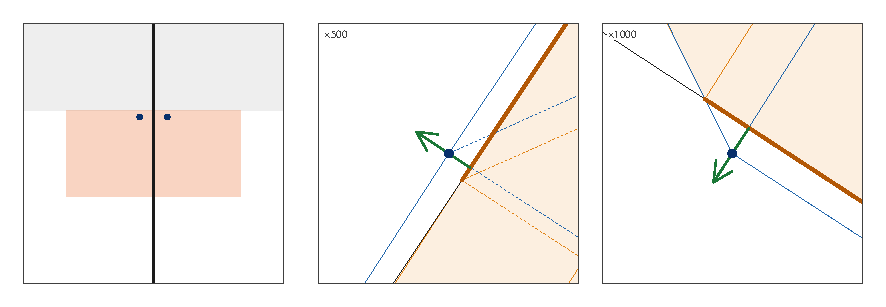
\includegraphics[width=\linewidth]{figures/pentagon-support}
\caption{The two sides of the edge-on line near the pentagon configuration. Left: the pentagon cover's viewing parameters in the coordinates $(\eta,\xi)$, with $\eta\in[-3/64,3/64]$ horizontally and $\xi\in[-1/16,1/32]$ vertically: \fc{Pentagon}{the covered rectangle $|\eta|\le1/32$, $-1/32\le\xi\le0$ (red-orange)}, \fc{Grey}{the views beyond the viewing triangle, $\xi>0$ (grey)}, the edge-on line $\eta=0$ (black) and two examples (dots) at $(\eta,\xi)=(-1/200,-1/400)$ and $(1/200,-1/400)$, both with the rotation $\mathbf r=(1/1000,0,0)$. Middle and right: their shadows near the protruding plug vertex, enlarged $500$ and $1000$ times, with the \fc{Hole}{hole (orange)} and the \fc{Plug}{plug (blue)} as in \cref{fig:global-examples} and a supporting line of the hole's shadow that \fc{Vertex}{this vertex (dark blue dot)} lies beyond. On the two sides, different plug vertices protrude beyond different hole edges.}
\label{fig:pentagon-support}
\end{figure}

\begin{proposition}[The pentagon neighbourhood]\label{prop:pentagon-neighbourhood}
  Every configuration $c\in D$ with $|\eta|\le1/32$, $-1/32\le\xi\le0$ and
  $\lVert\mathbf r\rVert_\infty\le1/16$ is a touch configuration if
  $\mathbf r=\mathbf0$ and a poke configuration otherwise.
\end{proposition}
\begin{proof}
  As for \cref{prop:square-neighbourhood}, using \cref{lem:point-coverage}
  and \cref{lem:zoom-lemma}; every cell's witness is a gap polynomial.
\end{proof}

\subsection{A neighbourhood of all aligned configurations}\label{subsec:ranges-and-remaining-touch-configurations}

The square and pentagon covers, together with the 30 covers of the Local
component, give a uniform neighbourhood of all aligned representatives.
Recall that a configuration lies in the range of the collection when the
collection accepts every search box in some neighbourhood of it
(\cref{def:range-of-a-component}). Write $\Delta$ for the viewing triangle
\cref{eq:viewing-triangle}, $W_0=[0,2/3]\times[0,2/5]$ for the viewing
rectangle of $B_0$, and $\delta_0=1/200$ for the smallest rotation bound
among the 32 covers of aligned configurations. Each of these covers has a
set of viewing parameters: a rectangle, or, for the pentagon cover, the
half-strip $|\eta|\le1/32$, $\xi\ge-1/32$ of its acceptance test (the upper
bound on $\xi$ is dropped because configurations with $\xi>0$ lie outside
$D$). Each cover contains every configuration whose viewing parameters lie
in its set and whose rotation satisfies
$\lVert\mathbf r\rVert_\infty\le\delta_0$. Shrink each set by $\beta=1/4096$ in
the maximum norm, except along the sides of $W_0$ (the half-strip has no
upper side to shrink). An
exact computation, bisecting $W_0$ and comparing endpoints in
$\mathbb Q(\sqrt5)$, shows that the shrunk sets still cover $\Delta$; without
the margin of $1/1024$ around each Local rectangle, which makes neighbouring rectangles overlap, this would
fail.

\begin{proposition}[A neighbourhood of all aligned representatives]\label{prop:aligned-neighbourhood}
  For every $(s_0,t_0)\in\Delta$, some cover of aligned configurations contains
  every configuration $[s,t,\mathbf r]\in B_0$ with
  $\max\{|s-s_0|,|t-t_0|\}\le\beta$ and $\lVert\mathbf r\rVert_\infty\le\delta_0$. Every
  such configuration in $D$ is a touch configuration when $\mathbf r=\mathbf0$ and a
  poke configuration otherwise. In particular, the union
  \begin{equation}\label{eq:aligned-neighbourhood-range}
    \bigcup_{(s_0,t_0)\in\Delta}\bigl\{[s,t,\mathbf r]\in B_0:
      \max\{|s-s_0|,|t-t_0|\}<\beta,\ \lVert\mathbf r\rVert_\infty<\delta_0\bigr\}
  \end{equation}
  lies in the collection's range.
\end{proposition}
\begin{proof}
  The pair $(s_0,t_0)$ lies in the shrunk set of some cover, so the
  maximum-norm ball of radius $\beta$ around it, cut to $W_0$, lies in that
  cover's set of viewing parameters. The geometric claim follows from
  \cref{prop:soundness-of-the-local-component,prop:square-neighbourhood,prop:pentagon-neighbourhood}.

  For the range, let $c$ lie in the union \cref{eq:aligned-neighbourhood-range}.
  It has a neighbourhood in $B_0$ inside one of the closed sets just
  described, and hence inside the covered set of one cover. Every search
  box contained in that neighbourhood lies in the covered set, so the
  cover's exact inclusion test accepts it.
\end{proof}

Because of the overlaps, the conclusion does not depend on where the
boundaries of the covers lie relative to the halving lines of the search,
and every aligned representative lies in the range, even on a boundary of
the viewing triangle.

\paragraph{Remaining touch configurations.}
With the Global and Local components and these two covers, the
unresolved boxes no longer concentrate around aligned configurations.
They concentrate instead along two segments of configurations in which the
plug and the hole have different orientations but their shadows still
touch (\cref{fig:arcs-remaining}). We describe them and the covers along
them in \cref{sec:arc-configurations}.

\begin{figure}[htbp]
\centering
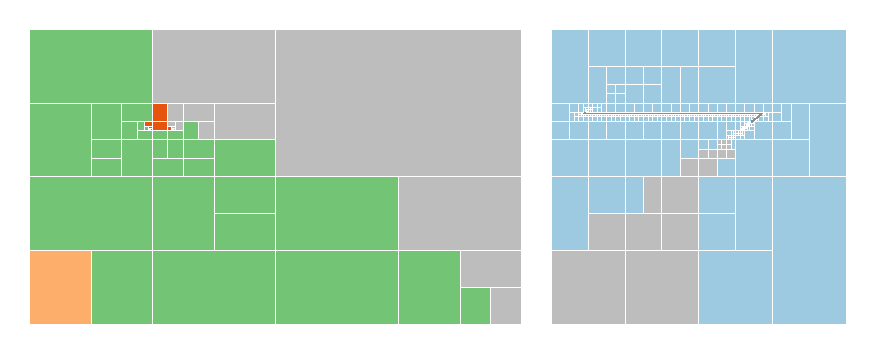
\includegraphics[width=\linewidth]{figures/arcs-remaining}
\caption{With the square and pentagon covers added. Left: the plane $\mathbf r=\mathbf 0$ of \cref{fig:exotic-directions}, now eliminated entirely, near the corner by \fc{Square}{the square cover (light orange)} and near the edge-on point by \fc{Pentagon}{the pentagon cover (red-orange)}. Right: a plane of non-aligned configurations with $t=0$, with $s\in[3/16,5/8]$ horizontally and a rotation parameter $\theta\in[-5/16,1/8]$ vertically (it is the plane $\Pi_1$ of \cref{sec:arc-configurations}). Unresolved pieces (black) remain along two segments that meet at $s=1/2$.}
\label{fig:arcs-remaining}
\end{figure}
